\documentclass[12pt,a4paper]{article}

% Packages
\usepackage[margin=1in,left=1.5in]{geometry}
\usepackage{times}
\usepackage{setspace}
\usepackage{titlesec}
\usepackage[titles]{tocloft}
\usepackage{fancyhdr}
\usepackage{graphicx}
\usepackage{array}
\usepackage{booktabs}

% Page style
\pagestyle{fancy}
\fancyhf{}
\fancyfoot[C]{\thepage}
\renewcommand{\headrulewidth}{0pt}

% Section formatting
\titleformat{\section}{\normalfont\Large\bfseries}{\thesection}{1em}{}

% Table of contents formatting
\renewcommand{\cfttoctitlefont}{\hfill\Large\bfseries}
\renewcommand{\cftaftertoctitle}{\hfill}
\renewcommand{\cftsecfont}{\normalfont}
\renewcommand{\cftsecpagefont}{\normalfont}
\setlength{\cftbeforesecskip}{5pt}

\begin{document}

\begin{titlepage}
    \begin{figure}[ht!]
        \centering
        
\includegraphics[height=2cm]{images/yu-logo.png}
    \end{figure}
    \vspace{.5cm}
    \centering{{College of Engineering and Architecture} \par}

    \vfill

    \centering
    {\LARGE\bfseries Project Proposal\par}
    \vspace{.5cm}
    {\large Bachelor of Science in Software and Network Engineering\par}
    \vfill
    \begin{singlespace}
    \setstretch{1.2}
    \LARGE
    Muwaqqit:\\An Elegant yet Simple Calendar Manager
    \end{singlespace}
    \vspace{2cm}

    \vfill
    
    \begin{center}
        \setlength{\fboxsep}{10pt}
        \setlength{\fboxrule}{1pt}
        \fbox{%
        \begin{tabular}{p{0.45\linewidth}p{0.45\linewidth}}
            \multicolumn{2}{c}{\textbf{Group Project Submission}} \\
            \midrule
            \textbf{Student Names} & \textbf{Student IDs} \\
            \midrule
            YAZED ALKHALAF & 202211123 \\
            SAIMAN TAKLAS & 202021400 \\
            AFFAN MOHAMMAD & 202211086 \\
            ALI BA WAZIR & 202211018 \\
            \midrule
            \multicolumn{2}{l}{\textbf{Submission Date}: 2 May 2024} \\
            \multicolumn{2}{l}{\textbf{Supervised By}: Dr. Inaya Allah} \\
        \end{tabular}%
        }
        \end{center}

    \vfill
    
    First Semester 2024--2025
\end{titlepage}

% Table of Contents
\tableofcontents
\clearpage

% Main content
\pagenumbering{arabic}
\doublespacing

\section{Background of the Project}

As the world is moving towards globalizing, effective time management is becoming very important. Considering how everything seems to be rushing in today's world, there is a high requirement for an effective user-friendly time management tool. Paper-based calendars have been used for addressing the complexities of managing multiple schedules across various aspects of life such as work, school, and personal commitments. However, they often fall short in providing a comprehensive solution to modern scheduling challenges.

The introduction of the digital calendar has somewhat solved this problem but still, users face a lot of issues in keeping their calendars up-to-date and synchronized. There are still few people that manually input events into their calendars. This could be really tiring, especially when dealing with multiple calendars.

Moreover, the rise of instant messaging platforms like WhatsApp has changed the way we communicate and plan events. Mostly, important dates and appointments are discussed informally leading to a disconnect between where the information is initially shared and where it needs to be recorded for effective time management.

To address these challenges, we are planning an application called \textit{Muwaqqit}, which aims to revolutionize how people manage their time and schedules in the digital age.

\section{Problem Statement}

The core problem that Muwaqqit addresses is the inefficient and potential conflicts in managing the personal and professional schedules in a globalized world, especially:

\begin{enumerate}
    \item Users struggle to keep their calendars up-to-date with information from various sources, particularly from informal mediums of communication such as WhatsApp.
    \item They manually add the events to the calendar which is time consuming and error-prone.
    \item Multiple calendars (work, school, and personal) create complexity and major risk of conflicts.
    \item There is a lack of seamless integration with popular communication platforms.
    \item High risk of missing events due to the distribution of information in many calendars and data sources.
    \item Because fragmented information can result in disarray and missed appointments, users frequently rely on multiple platforms for scheduling, including email, messaging apps, and paper calendars.
\end{enumerate}

\section{Objectives of the Project}

The main objectives of Muwaqqit are:

\begin{itemize}
    \item To develop an intelligent calendar management system that automatically extracts events from the communication channels and adds them to the user's main calendar.
    \item To create a user friendly interface that allows users to automatically add events to the calendar.
    \item To implement smart resolution system that notifies users of scheduling conflicts and provides easy options for resolution.
    \item To integrate all the calendars into Muwaqqit's single calendar view to make viewing and managing all the events easy.
    \item To prioritize and automatically schedule daily routines such as waking time, sleeping time and prayer time.
    \item To significantly reduce the time users spend on manual calendar management.
\end{itemize}

\section{Significance of the Project}

Muwaqqit endeavours to solve problems and its significance can be summarized in the following:

\begin{enumerate}
    \item \textbf{Time is Money}: Time is the only asset you can't get more of, it is being consumed til the last day of your life.
    \item \textbf{Prayer First Calendar}: Prayer times come first, then your daily scheduled items.
\end{enumerate}

\section{Scope of the Project}

Muwaqqit is not just another calendar application; it's a comprehensive time management tool designed to aggregate and optimize your existing calendars and data sources. The scope of the project includes:

\begin{itemize}
    \item Development of an iOS application as the primary platform.
    \item Integration with calendars using CalDAV.
    \item WhatsApp message parsing for event extraction (subject to technical feasibility).
    \item Target audience: Busy professionals, students, and anyone juggling multiple schedules.
    \item User testing phase to ensure ease of use and effectiveness.
\end{itemize}

Our testing methods will include:
\begin{itemize}
    \item Beta testing with a diverse group of users.
    \item Analytics to track user behavior and app performance.
\end{itemize}

\section{Limitations of the Project}

Nothing is perfect, and our project is not a outlier. The limitations we have figured out about it are as follows:

\begin{itemize}
    \item WhatsApp integration allows the app to read the users messages, so it would be hard to prove privacy hasn't been breached.
    \item WhatsApp integration might not always be there, they are a third-party.
    \item Learning new technologies for iOS development might require more time than anticipated.
    \item Accuracy of our algorithms to detect keywords indicating an event agreement has happened, especially for languages other than English.
    \item Time and manpower constraints may limit the number of features we can implement.
    \item Dependency on third-party calendar APIs and their limitations.
\end{itemize}

\section{Project Plan}

Our project plan can be illustrated in the following gantt chart, \textbf{Figure \ref{fig:project-gantt-chart}}.

\begin{figure}[!h]
    \centering
    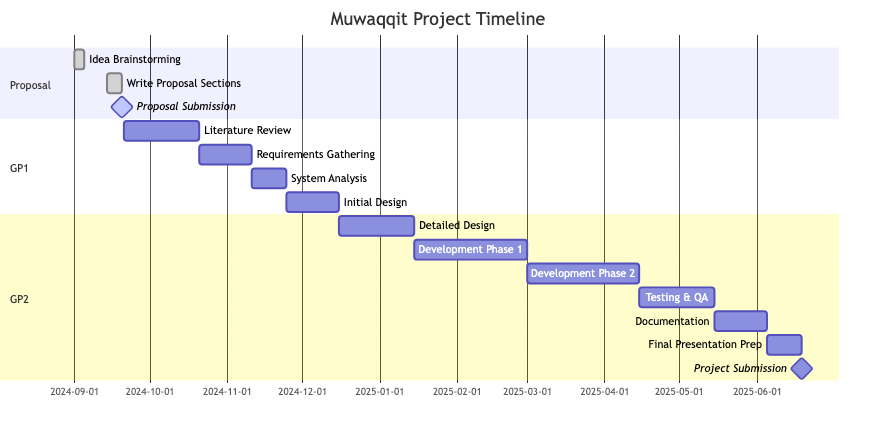
\includegraphics[width=\textwidth]{images/gantt.png}
    \caption{Project Gantt Chart}
    \label{fig:project-gantt-chart}
\end{figure}

\section{Literature Review}

In developing Muwaqqit, we have drawn inspiration from and built upon existing research and products in the field of intelligent calendar management. Some key references include:

\begin{itemize}
    \item \textbf{Clockwise (https://www.getclockwise.com/):} A smart calendar assistant that optimizes schedules and manages team coordination. Clockwise's approach to intelligent time blocking and meeting optimization provides valuable insights for Muwaqqit's automated scheduling features.
    \item \textbf{Calendi (https://calendi.ai/):} Calendi describes itself as: ''Calendi is an AI calendar system. Use it for scheduling tasks, automating meetings, and witness the future of calendar.;;
    \item \textbf{Motion (https://www.usemotion.com/):} Motion’s Intelligent Calendar takes your meetings. Your tasks. Your to-do list. Your activities. And creates one perfect, optimized schedule to get it all done.
    \item \textbf{Dola AI (https://heydola.com/):}
    \item \textbf{Reclaim AI (https://reclaim.ai/):}
    \item \textbf{An Exploratory Study of Calendar Use:} "Prospective remembering is the use of memory for remembering to do things in the future, as different from retrospective memory functions such as recalling past events." \cite{tungare2008exploratorystudycalendaruse}
    \item \textbf{WhatsApp Integration:} Our research indicates that direct WhatsApp integration for event extraction has not been widely implemented in existing calendar applications, making this a unique feature of Muwaqqit.
\end{itemize}

\begin{figure}[!h]
    \centering
    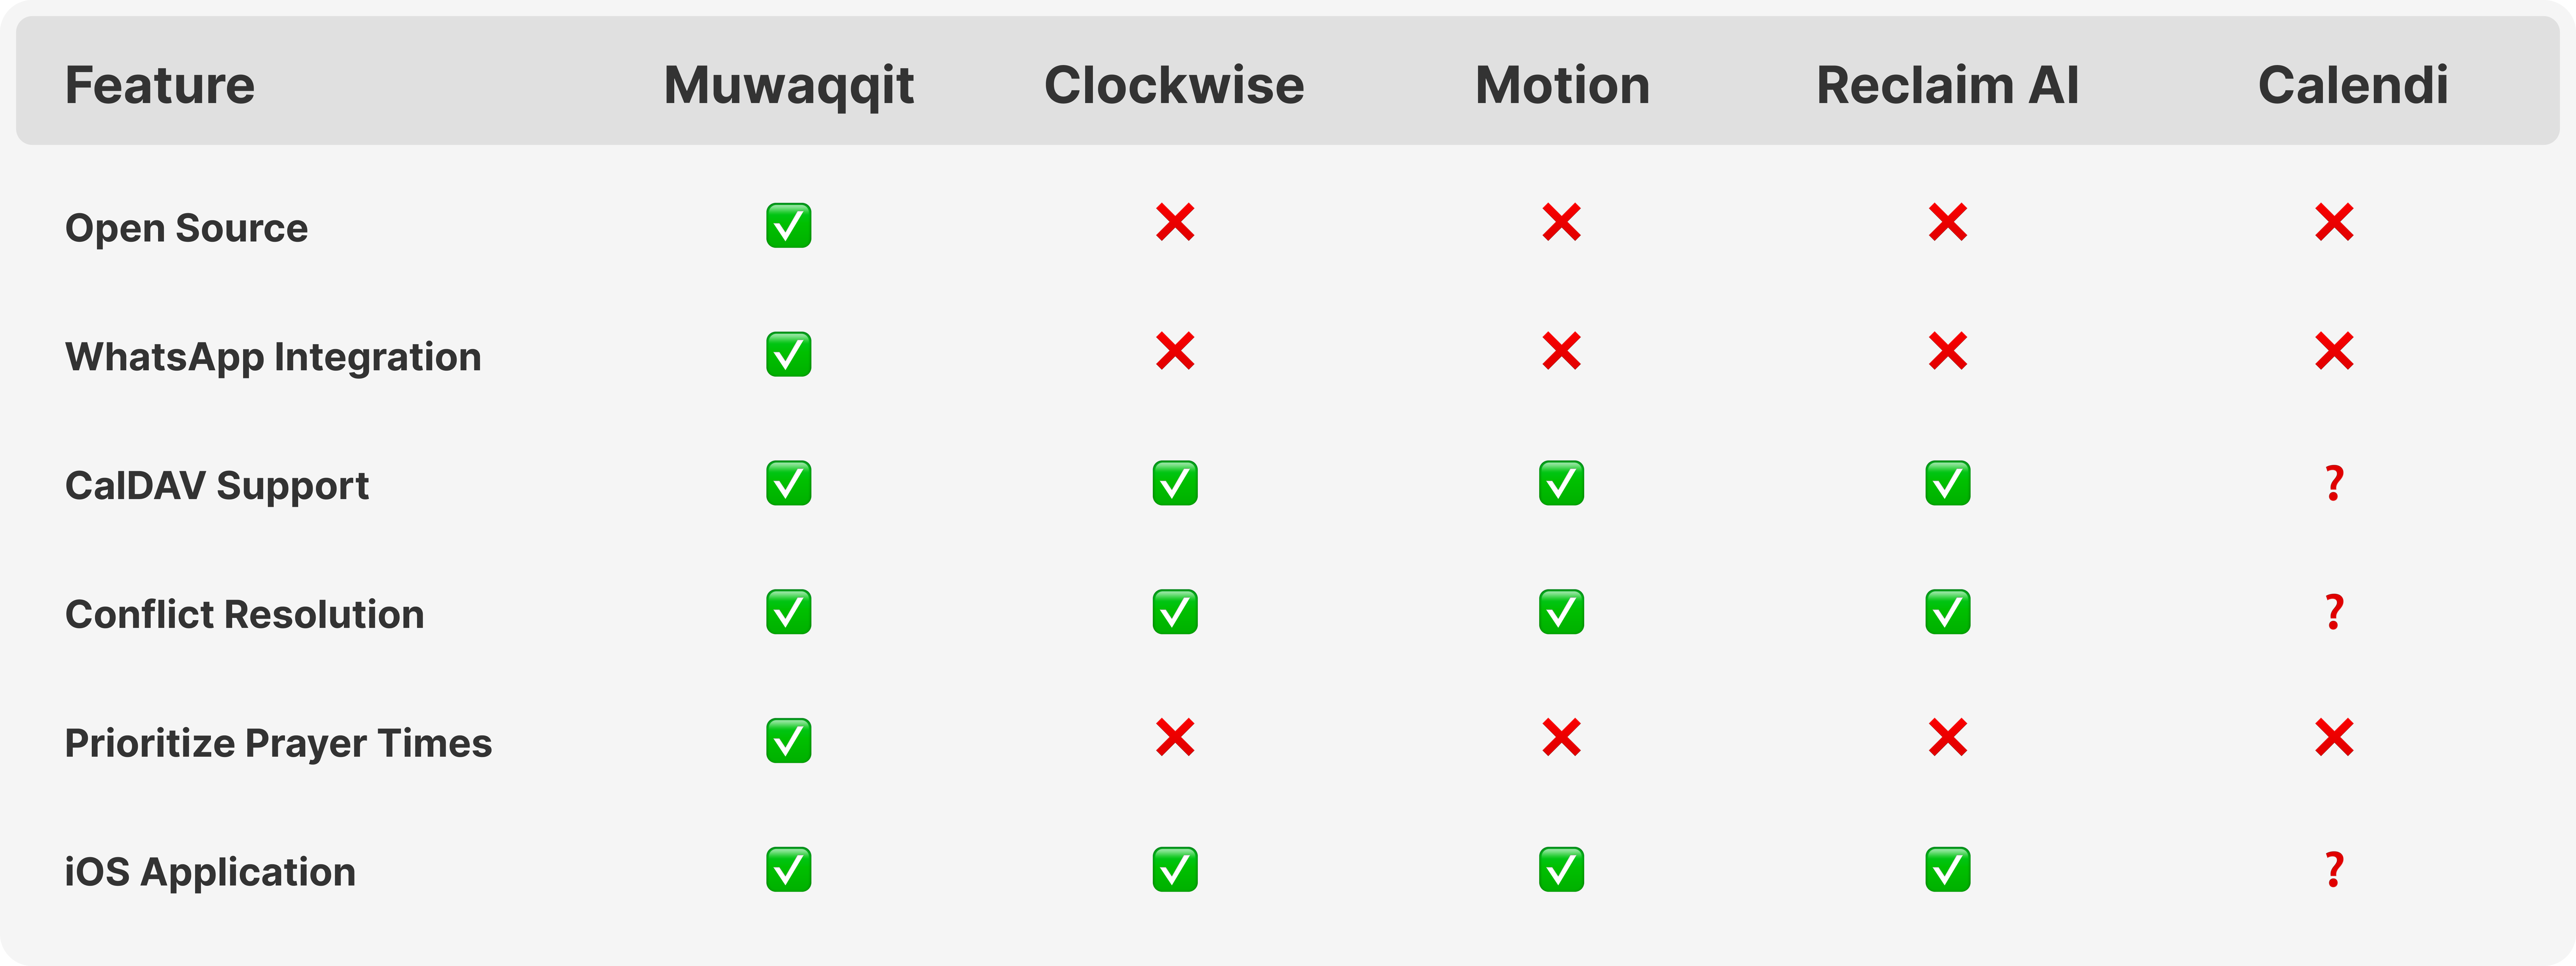
\includegraphics[width=\textwidth]{images/features-table.png}
    \caption{Feature Comparison Table}
    \label{fig:features-table}
\end{figure}

\noindent
Note: Y = Feature available, N = Feature not available, ? = Information unclear

\section{Technology and Outcomes}

The final product of this project will be:

\begin{itemize}
    \item An iOS application developed using Swift programming language.
    \item Backend services to handle data processing and integration with third-party APIs.
\end{itemize}

We will assess the feasibility of calendar integration and WhatsApp parsing throughout the development process, adjusting our approach as necessary to ensure the best possible user experience.

\section{Conclusion}

Muwaqqit aims to revolutionize personal time management by providing an intelligent, integrated solution to the challenges of modern scheduling. By leveraging seamless integration with communication platforms, we hope to significantly reduce the time and effort required for effective calendar management.

\newpage

\bibliography{references} 
\bibliographystyle{apalike}

\end{document}